%%%%%%%%%%%%%%%%%%%%%%%%%%%%%%%%%%%%%%%%%
% Arsclassica Article
% LaTeX Template
% Version 1.1 (10/6/14)
%
% This template has been downloaded from:
% http://www.LaTeXTemplates.com
%
% Original author:
% Lorenzo Pantieri (http://www.lorenzopantieri.net) with extensive modifications by:
% Vel (vel@latextemplates.com)
%
% License:
% CC BY-NC-SA 3.0 (http://creativecommons.org/licenses/by-nc-sa/3.0/)
%
%%%%%%%%%%%%%%%%%%%%%%%%%%%%%%%%%%%%%%%%%

%----------------------------------------------------------------------------------------
%	PACKAGES AND OTHER DOCUMENT CONFIGURATIONS
%----------------------------------------------------------------------------------------

\documentclass[
10pt, % Main document font size
a4paper, % Paper type, use 'letterpaper' for US Letter paper
oneside, % One page layout (no page indentation)
%twoside, % Two page layout (page indentation for binding and different headers)
headinclude,footinclude, % Extra spacing for the header and footer
BCOR5mm, % Binding correction
]{scrartcl}

%%%%%%%%%%%%%%%%%%%%%%%%%%%%%%%%%%%%%%%%%
% Arsclassica Article
% Structure Specification File
%
% This file has been downloaded from:
% http://www.LaTeXTemplates.com
%
% Original author:
% Lorenzo Pantieri (http://www.lorenzopantieri.net) with extensive modifications by:
% Vel (vel@latextemplates.com)
%
% License:
% CC BY-NC-SA 3.0 (http://creativecommons.org/licenses/by-nc-sa/3.0/)
%
%%%%%%%%%%%%%%%%%%%%%%%%%%%%%%%%%%%%%%%%%

%----------------------------------------------------------------------------------------
%	REQUIRED PACKAGES
%----------------------------------------------------------------------------------------

\usepackage[
nochapters, % Turn off chapters since this is an article        
beramono, % Use the Bera Mono font for monospaced text (\texttt)
eulermath,% Use the Euler font for mathematics
pdfspacing, % Makes use of pdftex’ letter spacing capabilities via the microtype package
dottedtoc % Dotted lines leading to the page numbers in the table of contents
]{classicthesis} % The layout is based on the Classic Thesis style

\usepackage{arsclassica} % Modifies the Classic Thesis package

\usepackage[T1]{fontenc} % Use 8-bit encoding that has 256 glyphs

\usepackage[utf8]{inputenc} % Required for including letters with accents

\usepackage{graphicx} % Required for including images
\graphicspath{{Figures/}} % Set the default folder for images

\usepackage{enumitem} % Required for manipulating the whitespace between and within lists

\usepackage{lipsum} % Used for inserting dummy 'Lorem ipsum' text into the template

\usepackage{subfig} % Required for creating figures with multiple parts (subfigures)

\usepackage{amsmath,amssymb,amsthm} % For including math equations, theorems, symbols, etc

\usepackage{varioref} % More descriptive referencing

%----------------------------------------------------------------------------------------
%	THEOREM STYLES
%---------------------------------------------------------------------------------------

\theoremstyle{definition} % Define theorem styles here based on the definition style (used for definitions and examples)
\newtheorem{definition}{Definition}

\theoremstyle{plain} % Define theorem styles here based on the plain style (used for theorems, lemmas, propositions)
\newtheorem{theorem}{Theorem}

\theoremstyle{remark} % Define theorem styles here based on the remark style (used for remarks and notes)

%----------------------------------------------------------------------------------------
%	HYPERLINKS
%---------------------------------------------------------------------------------------

\hypersetup{
%draft, % Uncomment to remove all links (useful for printing in black and white)
colorlinks=true, breaklinks=true, bookmarks=true,bookmarksnumbered,
urlcolor=webbrown, linkcolor=RoyalBlue, citecolor=webgreen, % Link colors
pdftitle={}, % PDF title
pdfauthor={\textcopyright}, % PDF Author
pdfsubject={}, % PDF Subject
pdfkeywords={}, % PDF Keywords
pdfcreator={pdfLaTeX}, % PDF Creator
pdfproducer={LaTeX with hyperref and ClassicThesis} % PDF producer
} % Include the structure.tex file which specified the document structure and layout

\usepackage{appendix}
% \usepackage{float}
% \usepackage{subfig}
\usepackage{caption}
\usepackage{subcaption}   % handles objects not covered by caption

\hyphenation{Fortran hy-phen-ation} % Specify custom hyphenation points in words with dashes where you would like hyphenation to occur, or alternatively, don't put any dashes in a word to stop hyphenation altogether

%----------------------------------------------------------------------------------------
%	TITLE AND AUTHOR(S)
%----------------------------------------------------------------------------------------

\title{\normalfont\spacedallcaps{BioMap}} % The article title

\subtitle{\normalfont\spacedlowsmallcaps{Prototype Report}}

\author{\spacedlowsmallcaps{Graeme Faul\textsuperscript{1} \& Gregory Linklater\textsuperscript{1}}} % The article author(s) - author affiliations need to be specified in the AUTHOR AFFILIATIONS block

\date{\today} % An optional date to appear under the author(s)

%----------------------------------------------------------------------------------------

\begin{document}

%----------------------------------------------------------------------------------------
%	HEADERS
%----------------------------------------------------------------------------------------

\renewcommand{\sectionmark}[1]{\markright{\spacedlowsmallcaps{#1}}} % The header for all pages (oneside) or for even pages (twoside)
%\renewcommand{\subsectionmark}[1]{\markright{\thesubsection~#1}} % Uncomment when using the twoside option - this modifies the header on odd pages
\lehead{\mbox{\llap{\small\thepage\kern1em\color{halfgray} \vline}\color{halfgray}\hspace{0.5em}\rightmark\hfil}} % The header style

\pagestyle{scrheadings} % Enable the headers specified in this block

%----------------------------------------------------------------------------------------
%	TABLE OF CONTENTS & LISTS OF FIGURES AND TABLES
%----------------------------------------------------------------------------------------

\maketitle % Print the title/author/date block

\setcounter{tocdepth}{2} % Set the depth of the table of contents to show sections and subsections only

\tableofcontents % Print the table of contents

\listoffigures % Print the list of figures

% \listoftables % Print the list of tables

%----------------------------------------------------------------------------------------
%	AUTHOR AFFILIATIONS
%----------------------------------------------------------------------------------------

{\let\thefootnote\relax\footnotetext{\textsuperscript{1} \textit{Department of Computer Science, Rhodes University, Grahamstown, South Africa}}}

%----------------------------------------------------------------------------------------

\newpage % Start the article content on the second page, remove this if you have a longer abstract that goes onto the second page

%----------------------------------------------------------------------------------------
%	CONTENT
%----------------------------------------------------------------------------------------

\section{Introduction} % (fold)
\label{sec:introduction}



% section introduction (end)

\section{Application Description} % (fold)
\label{sec:application_description}

% section application_description (end)

\section{Feedback} % (fold)
\label{sec:feedback}

\subsection{False Assumptions} % (fold)
\label{sub:false_assumptions}

After a conversation with \textit{Prof. Craig Peter} it became clear that our initial assumptions of how the system should operate were completely incorrect; in particular the following assumptions that we were operating under:

\begin{itemize}
\item The backend of the system would be completely separate to the existing system and would need to be built separately. This assumption was based on the fact that it was highly unlikely that the system administrators of the ADU would allow us (students) to interact and effect possibly breaking changes to a production system. Since the initial prototype was created, it seems that there will be a development system created that will be functionally equivalent to the production system for which we will be given API documentation and the relevant credentials to access. As of the time of writing, we have not yet been given such documentation which may or may not affect how the final product will operate when compared to this prototype document.
\item We would be able to add functionality to the existing system. This stems from the above point where we would be creating our own backend and could therefore define additional features. Ideas such as live communication with moderators regarding submissions, improved search functionality by indexing records through the use of ``tags'', the use of notifications and correcting database schema errors such as the restriction of three images to a submission are all therefore useless for the design of this application due to lack of access to the backend system. According to \textit{Prof. Peter} The restriction of the number of images per submission often leads to users submitting multiple records to cover all of the images the user has captured and the existing system has no way to link them. It is impossible to tell without more information, however this error is most likely an error in the database schema that has not been designed to conform to the 3\textsuperscript{rd} normal form.
\item The document containing a list of requests from \textit{Prof. Peter} showed additional features that were not supported by the existing system. Due to us operating under the above assumptions; this further reinforced that we would be able to implement these additional features when creating our own backend. Now that we know differently; it is clear that some of the requirements that were requested will be impossible to implement without modification of the existing system and we will therefore not be able to meet them.
\end{itemize}

The above false assuptions have therefore since required us to completely redesign the system which is what is reflected in this document.

% subsection false_assumptions (end)

\subsection{Changes to the System} % (fold)
\label{sub:changes_to_the_system}

From what we were able to salvage from our existing prototype, \textit{Prof. Peter} had the following comments:

\begin{itemize}
\item The use of icons to select the database on the home screen (Figure~\vref{wire:home}) seems to be a different approach; he seemed unsure of how it would work and stipulated that it would be difficult to use if icons for all of the databases were present on the page, as most of the users seem to restrict themselves to a handful of complimentary databases. We have therefore decided to keep the icon-based home screen -- as this decreases the amount of manual text entry on the part of the user when submitting a record -- and instead have added a process for adding icons to the home screen from the list of existing databases. Due to the fact that we have not yet recieved API documentation the list of databases; the list (Figure~\vref{wire:add_db}) will be built statically.
\item The addition of the ``My Records'' screen (Figure~\vref{wire:records_list}) received positive feedback as it seems that it is fairly difficult, when batch uploading a large amount images, to remember where exactly one is in the process. Initially the plan was have one screen that contained all the records submitted for all the databases the user contributes to, and records were distinguished by name, date and an icon showing which database the submission was contributing to.
\end{itemize}

Some of these changes have been reflected in this document and others have not due to time restrictions. The changes that are not reflected in this document will hopefully be present in the final product if there is sufficient time to include them.

% subsection changes_to_the_system (end)

% section feedback (end)

\section{Prototype} % (fold)
\label{sec:prototype}

% section prototype (end)

\section{Conclusion} % (fold)
\label{sec:conclusion}

% section conclusion (end)

\newpage

%----------------------------------------------------------------------------------------
%	BIBLIOGRAPHY
%----------------------------------------------------------------------------------------

% \renewcommand{\refname}{\spacedlowsmallcaps{References}} % For modifying the bibliography heading

% \bibliographystyle{apalike}

% \bibliography{sample.bib} % The file containing the bibliography

% \newpage

%----------------------------------------------------------------------------------------
% APPENDICES
%----------------------------------------------------------------------------------------

\begin{appendices}

\section{Wireframes} % (fold)
\label{sec:wireframes}

\subsection{Login} % (fold)
\label{sub:login}

\begin{figure}[htb]
\centering 
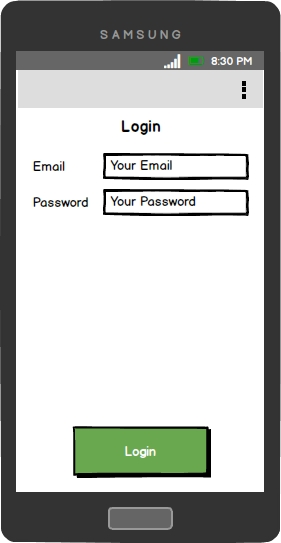
\includegraphics[width=.35\columnwidth]{LoginScreen} 
\caption{Login Screen Wireframe} % The text in the square bracket is the caption for the list of figures while the text in the curly brackets is the figure caption
\label{wire:login} 
\end{figure}

% subsection login (end)

\subsection{Home} % (fold)
\label{sub:home}

\begin{figure}[htb]
\centering 
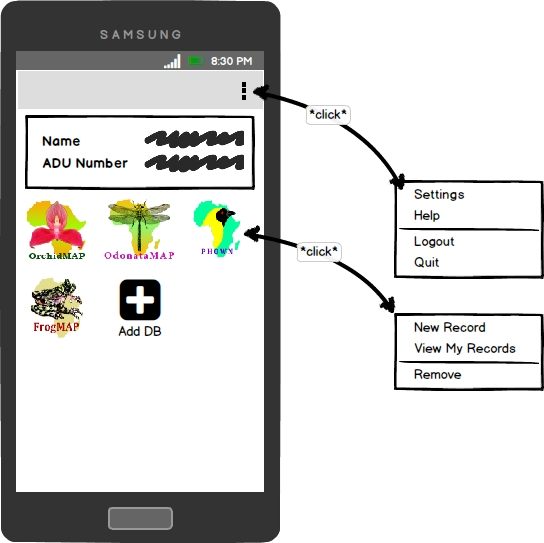
\includegraphics[width=.65\columnwidth]{HomeScreen} 
\caption{Home Screen Wireframe}
\label{wire:home} 
\end{figure}

\begin{figure}[htb]
\centering 
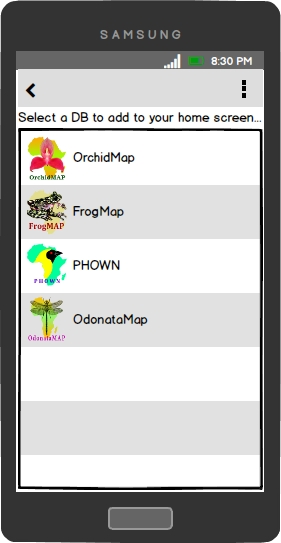
\includegraphics[width=.35\columnwidth]{AddDBScreen} 
\caption{Add Database Shortcut Screen Wireframe} 
\label{wire:add_db} 
\end{figure}

% subsection home (end)

\newpage

\subsection{Settings} % (fold)
\label{sub:settings}

\begin{figure}[htb]
\centering 
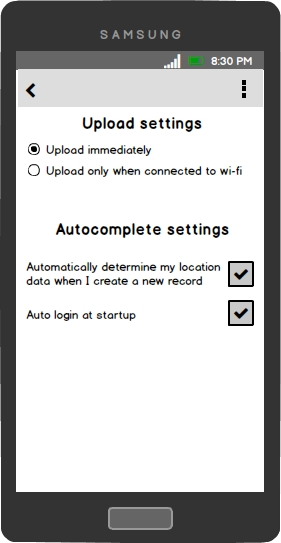
\includegraphics[width=.35\columnwidth]{SettingsScreen} 
\caption{Settings Screen Wireframe} 
\label{wire:settings} 
\end{figure}

% subsection settings (end)

\newpage

\subsection{Help} % (fold)
\label{sub:help}

\begin{figure}[h]
\centering
\begin{subfigure}{.5\columnwidth}
  \centering
  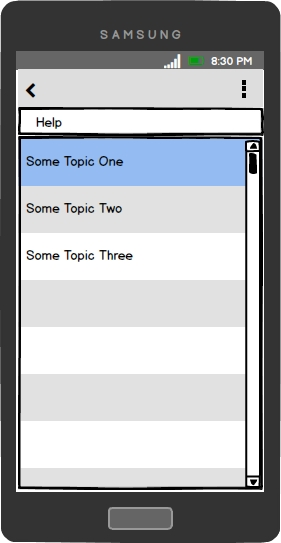
\includegraphics[width=.8\textwidth]{HelpHomeScreen}
  \caption{Select Help Topic Screen}
  \label{wire:help_home}
\end{subfigure}%
\begin{subfigure}{.5\columnwidth}
  \centering
  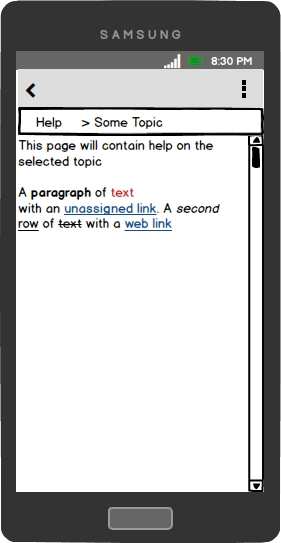
\includegraphics[width=.8\textwidth]{HelpTopicScreen}
  \caption{View Help Topic Screen}
  \label{wire:help_topic}
\end{subfigure}
\caption{User Help List and Detail Wireframes}
\label{wire:help}
\end{figure}

% subsection help (end)

\newpage

\subsection{Record} % (fold)
\label{sub:record}

\begin{figure}[h]
\centering
\begin{subfigure}[b]{.475\textwidth}
  \centering
  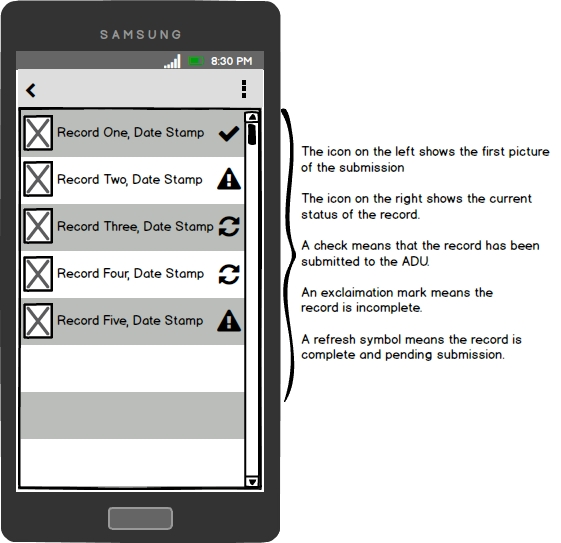
\includegraphics[width=.8\textwidth]{ViewRecordsScreen}
  \caption{Record List Screen Wireframe}
  \label{wire:records_list}
\end{subfigure}
\begin{subfigure}[b]{.475\textwidth}
  \centering
  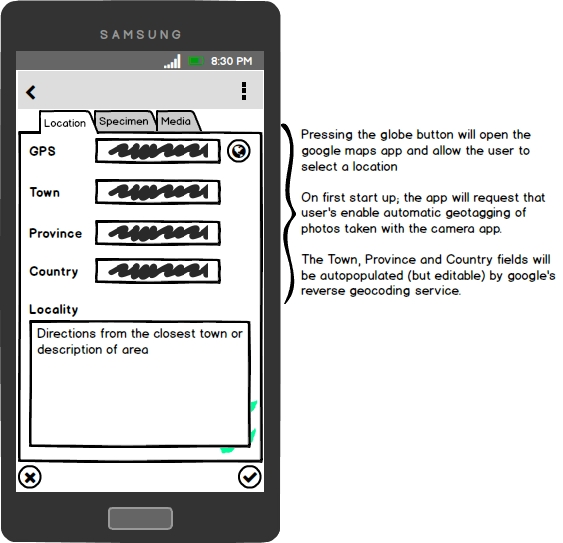
\includegraphics[width=.8\textwidth]{AddEditRecordLocation}
  \caption{Record Location Tab Wireframe}
  \label{wire:record_loc}
\end{subfigure}
\quad
\begin{subfigure}[b]{.475\textwidth}
  \centering
  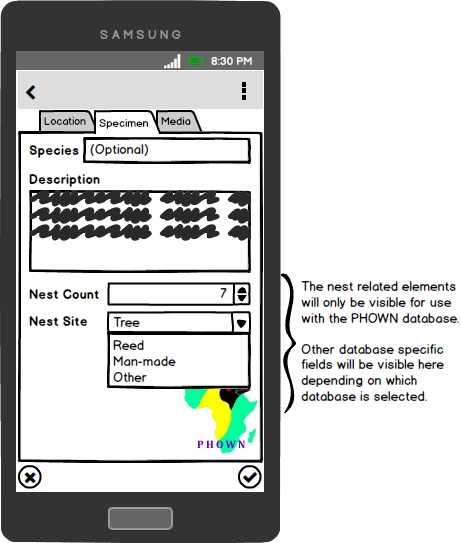
\includegraphics[width=.75\textwidth]{AddEditRecordSpecimen}
  \caption{Record Specimen Tab Wireframe}
  \label{wire:record_specimen}
\end{subfigure}
\begin{subfigure}[b]{.475\textwidth}
  \centering
  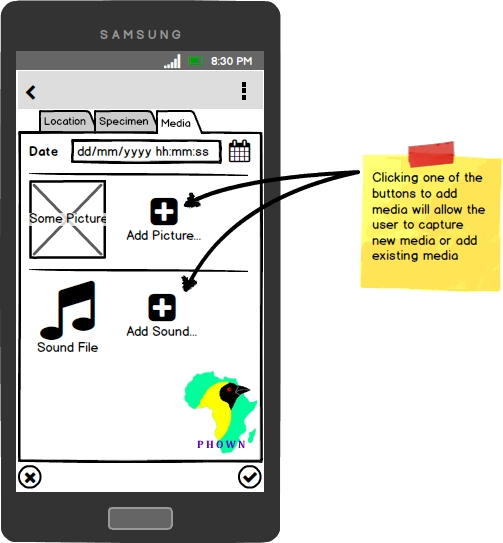
\includegraphics[width=.8\textwidth]{AddEditRecordMedia}
  \caption{Record Media Tab Wireframe}
  \label{wire:record_media}
\end{subfigure}
\caption{Record List and Detail Wireframes}
\label{wire:help}
\end{figure}

% subsection record (end)

% section wireframes (end)

\end{appendices}

\end{document}